\chapter{Lecture 25 - Solving IVPs with Runge-Kutta Methods}
\label{ch:lec25n}
\section{Objectives}
The objectives of this lecture are to:
\begin{itemize}
\item Qualitatively motivate and describe the derivation of Runge-Kutta methods
\item Do some example problems
\end{itemize}
\setcounter{lstannotation}{0}

\section{Runge-Kutta Methods}
Runge-Kutta (RK) methods are a family of single-step numerical methods for solving first order initial value problems.
\begin{align*}
y^{\prime} &= f(t,y) \\
y(0) &= y_0
\end{align*}
The basic idea stems from that of Euler's methods where we approximated $y_{n+1}$ based on $y_n$, the slope, $y^{\prime}=f(t,y)$, and the step size, $h$.
\begin{equation*}
y_{n+1} = y_n + f(t,y)h
\end{equation*}
This can be expressed more exactly in terms of integrals:
\begin{equation*}
y_{n+1}=y_n+\int y^{\prime} \ \text{dt} = y_n+\int_{t_{n}}^{t_{n+1}}  f(t) \ \text{dt}
\end{equation*}
In your earlier classes in ordinary differential equations, this method of integrating to ``un-do'' the derivative is a standard solution method for separable initial value problems:
\begin{equation*}
\frac{dy}{dt} = y^{\prime} = \frac{h(t)}{g(y)} \Rightarrow \int g(y) \ \text{dy} = \int h(t) \ \text{dt}
\end{equation*}
For the simple case where $g(y) = 1$ and we integrate over one time step we get:
\begin{equation*}
\int_{y_{n}}^{y_{n+1}} 1 \ \text{dy} \rightarrow y_{n+1} = y_n + \int_{t_n}^{t_{n+1}} f(t)\ \text{dt}
\end{equation*}
Let us generalize a bit further and consider first order IVPs in the form:
\begin{equation}
y_{n+1} = y_n + \int_{t_n}^{t_{n+1}} f(t,y) \ \text{dt}
\label{eq:lec25n-1}
\end{equation}
and propose that we use \emph{quadrature} instead of exact integration.  Now we can re-write Equation \ref{eq:lec25n-1} as:\marginnote{\textbf{Note:} With this notation, $y_n = y(t_n)$ and $y_{n+1} = y(t_{n+1})$.}
\begin{equation}
y_{n+1} = y_n + h \sum\limits_{i=1}^{s} b_i f(t_n + c_ih,y(t_n+c_ih))
\end{equation}
where $h$ is like the scaling term, $\sfrac{b-a}{2}$, in Gauss quadrature, $b_i$ are the weights, and $c_i$ are the sample points.  We constrain $c_i \in [0,1]$ so that $t_n \le (t_n+c_ih) \le t_{n+1}$. \marginnote[-0.5cm]{\textbf{Note:} To prevent confusion with Gauss quadrature, from now on, we will refer to $c_i$ as the \emph{RK nodes} and $b_i$ as the \emph{RK weights}.}

\newthought{One problem with} this approach is that we do not know the value of $y(t_n+c_jh)$.  In RK methods, we will approximate these points between $y_n$ and $y_{n+1}$ as follows:
\begin{align*}
\xi_{\nu} &= y_n + h\sum\limits_{i=1}^{s}a_{\nu,i}f(t_n+c_ih,\xi_i) \\
y_{n+1} &= y_n + h\sum\limits_{i=1}^{s}b_i f(t_n+c_ih,\xi_i)
\end{align*}
The number of sample points, $s$, is referred to as the number of \emph{stages} and the elements $a_{\nu,i}$ are customarily arranged into a square matrix, called the \emph{RK matrix}.  As an example, for a 2-stage system, we can write out these equations fully as:\marginnote[0.75cm]{\textbf{Note:} Notice that the top equation is, in general, non-linear and must be solved iteratively using one of the methods we learned for non-linear systems of equations.  If the RK matrix is strictly lower triangular---i.e. only non-zero below the main diagonal---then the values for $\xi_i$ can be solved without iteration.}
\begin{align*}
\bracketVectorstack{\xi_1 \\ \xi_{2}} &= y_n + h\bracketMatrixstack{a_{11} & a_{12} \\ a_{21} & a_{22}} \bracketVectorstack{f(t_n+c_1h,\xi_1) \\ f(t_n+c_2h,\xi_2)} \\
y_{n+1} &= y_n + h \bracketMatrixstack{b_1 & b_2}\bracketVectorstack{f(t_n+c_1h_1,\xi_1) \\ f(t_n+c_2h,\xi_2)}
\end{align*}
\begin{marginfigure}
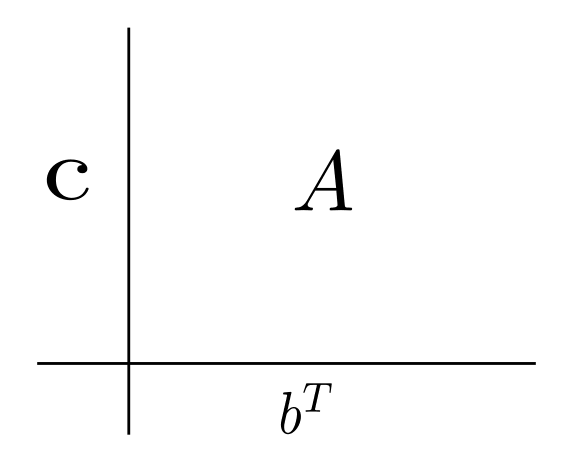
\includegraphics{lec25n-butcher-tableau.png}
\caption{Schematic of a Butcher Tableau.}
\label{fig:lec25n-butcher-tableau}
\end{marginfigure}
For an \emph{explicit} RK method, the RK matrix is strictly lower triangular.  The values of the RK weights, RK nodes, and entries in the RK matrix are customarily organized as a Butcher Tableau\cite{butcher2016numerical} as illustrated in Figure \ref{fig:lec25n-butcher-tableau}.  

In this class we will not derive any RK methods from scratch.  Still, we can make some general observations about RK methods:
\begin{enumerate}
\item The order of convergence for explicit RK methods is equal to the number of stages for $s<=4$.  RK methods with greater than 4\textsuperscript{th}-order convergence have been derived, but in those cases the number of stages, $s$, is greater than the order of convergence.

\item The sum of each row in the RK matrix is equal to the corresponding RK node.
\item the sum of the RK weights is equal to 1.
\end{enumerate}

\newthought{From this perspective} the modified Euler's method presented in the last lecture is equivalent to a 2-stage RK method. The RK nodes, RK weights, and RK matrix are shown below:
\begin{equation*}
c = \bracketVectorstack{0 \\ 1}, \ \ b^{T} = \bracketMatrixstack{\sfrac{1}{2} & \sfrac{1}{2}}, \ \ A = \bracketMatrixstack{0 & 0 \\ 1 & 0}
\end{equation*}
and the Butcher Tableau is shown in Table \ref{tab:lec25n-mem-tableau}.
\begin{margintable}
\begin{tabular}{c|cc}
0 & 0 & 0 \\
1 & 1 & 0 \\ \hline
  & $\sfrac{1}{2}$ & $\sfrac{1}{2}$ \\
\end{tabular}
\caption{Butcher Tableau for the modified Euler's method.}
\label{tab:lec25n-mem-tableau}
\end{margintable}

\section{MATLAB Implementation of RK Methods}

In this section I will present and explain three successive MATLAB implementations of an RK method.  The goal for this implementation is clarity and generality, not performance.  Students who are interested in achieving greater performance are encouraged to find optimizations sometime \emph{after} they fully understand what is shown here.

\subsection{2\textsuperscript{nd}-Order RK Method, Scalar 1\textsuperscript{st}-Order Equation}
We will start with an implementation of the modified Euler's method cast as an RK method for a scalar differential equation of 1\textsuperscript{st}-order.  The first portion of the function is shown in the listing below. Here we document the input and output variables; define variables to hold the RK matrix, RK weights, and RK nodes; and allocate a vector for the solution.

\begin{lstlisting}[style=myMatlab,name=lec25n-1]
function y = odeRK2(f,a,b,N,yINI)
% function y = odeRK2(f,a,b,h,yINI)
% y = solution
% f = function handle for y'
% a,b = interval for solution
% N = number of steps between a and b (inclusive)
% yINI = initial value for the solution

A = [0 0;
    1 0]; % RK matrix
B = [0.5 0.5]; % weights
c = [0 1]';% sample points
stages = 2;

x = linspace(a,b,N);
y = nan(1,N);
y(1) = yINI;
h = x(2)-x(1);
\end{lstlisting}

\noindent Now we will calculate RK solution process:\marginnote{

\vspace{0.5cm}

\noindent\ref{lst:ann25n-1} A new array of slopes, one element for each stage, will be needed at each time step.

\vspace{0.3cm}

\noindent\ref{lst:ann25n-2} This nested for loop calculates:
$$\xi_{s} = y_n + h\sum\limits_{i=1}^{s-1} a_{s,i}f(t_n+c_ih,\xi_{i})$$
for each value of $s$.  The upper limit of the summation index, $s-1$, is due to the fact that this is an explicit method and the RK matrix is strictly lower triangular.

\vspace{0.2cm}

\noindent\ref{lst:ann25n-3} This loop calculates:
$$y_{n+1} = y_n + h\sum\limits_{i=1}^{s}b_if(t_n+c_ih,\xi_i)$$

}
\begin{lstlisting}[style=myMatlab,name=lec25n-1]
for t = 1:(N-1)
    Xi = nan(1,stages); /*!\annotation{lst:ann25n-1}!*/
    
    for s = 1:stages
       Xi(s) = y(t); /*!\annotation{lst:ann25n-2}!*/
       for i = 1:(s-1)
          Xi(s) = Xi(s) + ...
              h*A(s,i)*f(x(t)+c(i)*h,Xi(i)); 
       end
    end
    
    y(t+1) = y(t);
    for i = 1:stages
       y(t+1) = y(t+1) + ...
           h*B(i)*f(x(t)+c(i)*h,Xi(i)); /*!\annotation{lst:ann25n-3}!*/
    end    
end
end
\end{lstlisting}

\newthought{We will use} this function to solve an example problem.

\vspace{0.25cm}

\noindent\textbf{Example \#1:} Solve the following initial value problem:
\marginnote{\textbf{Note:} It is worth emphasizing yet again the importance of testing a new method and/or a new implementation on a problem where you already know the solution.}
\begin{equation*}
y^{\prime} = \sfrac{x^2}{y}, \ \ y(0) = 2 
\end{equation*}
where the exact solution is: 
\begin{equation*}
y(x) = \left(\frac{2}{3}x^3 + 4\right)^{\sfrac{1}{2}}
\end{equation*}

\noindent In the listing below we set up the problem and invoke our 2\textsuperscript{nd}-order RK solver:
\begin{lstlisting}[style=myMatlab,name=lec25n-2]
clear
clc
close 'all'

%% Define the problem to be solved.
%%
% 
% $$y^{\prime} = x^2/y, \ \ y(0)=2$$
% 
f = @(x,y) (x.^2)./y; % y' = f(x,y)
yINI = 2; % y(0) = 2
y_exact = @(x) sqrt((2/3)*x.^3 + 4);
xMin = 0; xMax = 2.0;
x_gold = linspace(xMin,xMax,1000);

%% Invoke the solver
N = 30;
x = linspace(xMin,xMax,N);
y_RK2 = odeRK2(f,xMin,xMax,N,yINI);
\end{lstlisting}

\noindent Once the solution is complete we visualize the results.

\vspace{0.25cm}

\begin{lstlisting}[style=myMatlab,name=lec25n-2]
%% Plot the results
figure(1)
plot(x,y_RK2,'-b',...
    x_gold,y_exact(x_gold),'-.r',...
    'linewidth',3);
title("Solution with RK2 Method",'fontsize',14,...
    'fontweight','bold');
xlabel('X','fontsize',12,'fontweight','bold');
legend('RK2 Solution','Exact Solution','location','best');
grid on;
set(gca,'fontsize',10,'fontweight','bold');
\end{lstlisting}

\begin{marginfigure}
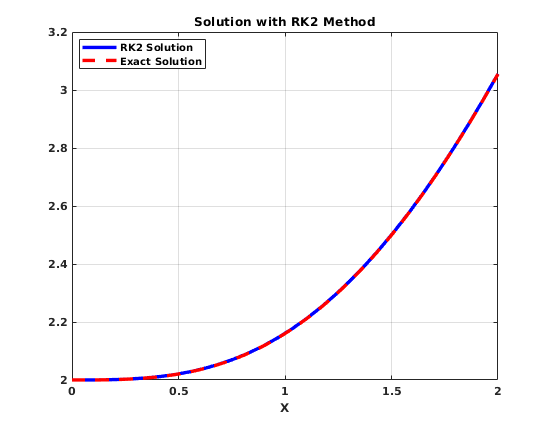
\includegraphics{lec25n-ex1.png}
\caption{Comparison between numeric and exact solution for Example \#1.}
\label{fig:lec25n-ex1}
\end{marginfigure}

\noindent A comparison between the numeric and exact solutions is shown in Figure \ref{fig:lec25n-ex1}. 

\newthought{While it seems} evident that the numeric solution is correct, plots of this sort are not adequate for verifying the correct performance of the numeric solver.  The numeric method should exhibit 2\textsuperscript{nd}-order convergence and we want to, somehow, verify this behavior.  The next MATLAB listing re-computes the numeric solution with successively smaller step-sizes.  For each solution, the relative error is computed in the 2-norm.  If the relative error is, indeed, proportional to $h^2$, then we can have more confidence that the algorithm is implemented correctly.  Figure \ref{fig:lec25n-ex1-conv} compares the relative error trend with what we would expect for a 2\textsuperscript{nd}-order convergent method.  The MATLAB code to carry out this task is shown in the next listing.
\begin{marginfigure}
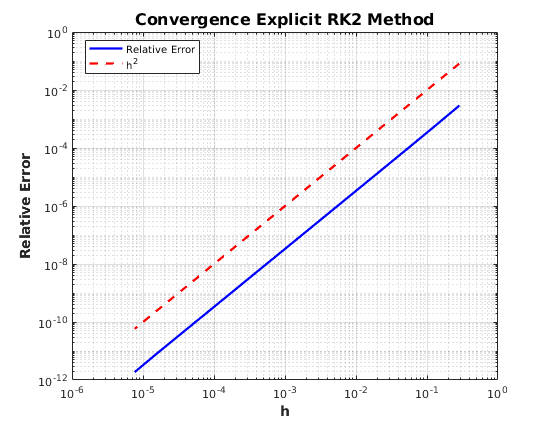
\includegraphics{lec25n-ex1-conv.png}
\caption{Convergence behavior of 2\textsuperscript{nd}-order RK method for Example \#1.}
\label{fig:lec25n-ex1-conv}
\end{marginfigure}
\setcounter{lstannotation}{0}
\marginnote{

\vspace{1.75cm}

\noindent \ref{lst:ann25n-1} Compute 2-norm of the error and normalize by the 2-norm of the exact solution to get the \emph{relative} error in the 2-norm.

\vspace{0.25cm} 

\noindent \ref{lst:ann25n-2} Create a vector proportional to $h^2$ to compare with the relative error.

}
\begin{lstlisting}[style=myMatlab,name=lec25n-2]
%% Convergence Test
N = 3:18;
t = length(N);
err_array = nan(1,t);
h_array = nan(1,t);
for s = 1:t
   Nx = 2^(N(s));
   x = linspace(xMin, xMax, Nx);
   h = x(2)-x(1);
   h_array(s) = h;
   y_ns = odeRK2(f,xMin,xMax,Nx,yINI);
   err_array(s) = norm(y_exact(x)-y_ns,2)./... /*!\annotation{lst:ann25n1-1}!*/
       norm(y_exact(x),2);
end

err_gage = h_array.^2;  /*!\annotation{lst:ann25n1-2}!*/

figure(2)
loglog(h_array,err_array,'-b',...
    h_array,err_gage,'--r','linewidth',2);
title("Convergence Explicit RK2 Method",...
    'fontsize',14,'fontweight','bold');
xlabel('h','fontsize',12,'fontweight','bold');
ylabel('Relative Error','fontsize',12,'fontweight','bold');
grid on
legend('Relative Error','h^2','location','best');
\end{lstlisting}

\subsection{Generalized Explicit RK Method for 1\textsuperscript{st}-Order Equation}

Instead of hard-coding the RK weights, sample points, and RK matrix into a solver, we can instead create a generalized solver that can use any explicit RK method where the aforementioned parameters are passed in via the Butcher tableau.  Consider the function shown in the MATLAB listing below:
\marginnote{

\vspace{3.5cm}

\noindent \ref{lst:ann25n2-1} The Butcher tableau is stored in a $(s+1) \times (s+1)$ matrix, where $s$ is the number of stages.  The layout is as shown in Figure \ref{fig:lec25n-butcher-tableau}.

}
\begin{lstlisting}[style=myMatlab,name=lec25n-3]
function y = odeExplicitRK(f,a,b,N,yINI,BT)
% function y = odeExplicitRK(f,a,b,h,yINI,BT)
% y = solution
% f = function handle for y'
% a,b = interval for solution
% N = number of steps between a and b (inclusive)
% yINI = initial value for the solution
% BT = Butcher Tableau

% Un-pack Butcher tableau parameters /*!\annotation{lst:ann25n2-1}!*/
s = length(BT)-1;
c = BT(1:s,1);
B = BT(s+1,2:end);
A = BT(1:s,2:end);
stages = s;

%% Carry out explicit RK method as specified
x = linspace(a,b,N);
y = nan(1,N);
y(1) = yINI;
h = x(2)-x(1);

for t = 1:(N-1)
    Xi = nan(1,stages);    
    for s = 1:stages
       Xi(s) = y(t);
       for i = 1:(s-1)
          Xi(s) = Xi(s) + ...
              h*A(s,i)*f(x(t)+c(i)*h,Xi(i)); 
       end
    end
    
    y(t+1) = y(t);
    for i = 1:stages
       y(t+1) = y(t+1) + h*B(i)*f(x(t)+c(i)*h,Xi(i)); 
    end    
end
end
\end{lstlisting}

We can use this generalized solver to repeat the calculation for Example \#1 as shown in the MATLAB listing below.

\begin{lstlisting}[style=myMatlab,name=lec25n-4]
%% Use Generalized Explicit RK method based on Butcher Tableau
% Construct Butcher tableau for 2nd-order RK method
s = 2;
BT = zeros(s+1,s+1);
C = [0; 1; 0];
B = [0 1/2 1/2];
A = [0 0;
    1 0;];
BT(:,1) = C;
BT(end,:) = B;
BT(1:s,2:end) = A;

%% Set parameters and invoke the solver
N = 30;
yINI = 2;
x = linspace(xMin,xMax,N);
y_RK2 = odeExplicitRK(f,xMin,xMax,N,yINI,BT);

%% Plot the results
figure(3)
plot(x,y_RK2,'-b',...
    x_gold,y_exact(x_gold),'-.r',...
    'linewidth',3);
title("Solution with RK2 Method",'fontsize',14,...
    'fontweight','bold');
xlabel('X','fontsize',12,'fontweight','bold');
legend('RK2 Solution','Exact Solution','location','best');
grid on;
set(gca,'fontsize',10,'fontweight','bold');
\end{lstlisting}

With this function, \emph{any} explicit RK method can be carried out; all that the user needs to do is to provide the corresponding Butcher tableau.

\subsection{Explicit RK Method for Systems of 1\textsuperscript{st}-Order Equations}

It should be clear to the reader that what we have done so far is not quite enough.  The method is only written to deal with first-order equations while, in general, our solver should be able to handle \emph{systems} of equations so higher-order IVPs can be solved.

\vspace{0.25cm}

\noindent\textbf{Example \#2:} Solve the following initial value problem using an explicit Runge-Kutta method.
\begin{equation*}
4y^{\prime \prime} + 4y^{\prime} + 17y = 0, \ \ y(0)=-1, \ \ y^{\prime}(0) = 2
\end{equation*}
The exact solution is:
\begin{equation*}
y(x) = e^{-\sfrac{x}{2}}\left[-\cos{(2x)} + \frac{3}{4}\sin{(2x)} \right]
\end{equation*}
To solve this equation we need to re-formulate the IVP as a first order system of equations:
\begin{align*}
y^{\prime \prime} &= -y^{\prime} - \frac{17}{4}y \\
w &= \bracketVectorstack{y \\ y^{\prime}}, \ \ dw = \bracketVectorstack{w(2) \\ -w(2) - \frac{17}{4}w(1)}
\end{align*}

\newthought{To handle this} situation, we will re-write the generalized Runge-Kutta ODE solver so that it can handle a system of equations.


\begin{lstlisting}[style=myMatlab,name=lec25n-5]
function y = odesExplicitRK(f,a,b,N,yINI,BT)
% function y = odeExplicitRK(f,a,b,h,yINI,BT)
% y = solution (vector)
% f = function handle for y'
% a,b = interval for solution
% N = number of steps between a and b (inclusive)
% yINI = initial value for the solution
% BT = Butcher Tableau

% Unpack Butcher tableau parameters
s = length(BT)-1;
c = BT(1:s,1);
B = BT(s+1,2:end);
A = BT(1:s,2:end);
stages = s;

%% Carry out explicit RK method on the system of equations
x = linspace(a,b,N);
sys_size = length(yINI);
y = nan(sys_size,N);
y(:,1) = yINI;
h = x(2)-x(1);
for t = 1:(N-1)
    Xi = nan(sys_size,stages);
    
    for s = 1:stages
       Xi(:,s) = y(:,t);
       for i = 1:(s-1)
          Xi(:,s) = Xi(:,s) + ...
              h*A(s,i)*f(x(t)+c(i)*h,Xi(:,i)); 
       end
    end
    
    y(:,t+1) = y(:,t);
    for i = 1:stages
       y(:,t+1) = y(:,t+1) + ...
           h*B(i)*f(x(t)+c(i)*h,Xi(:,i)); 
    end
    
end
end
\end{lstlisting}
\marginnote{ 

\vspace{-10.0cm}

\noindent \textbf{Note:} Readers are strongly encouraged to compare this implementation with the explicit RK solver for 1\textsuperscript{st}-order equations.  The dependent variable, $y$, is now a two-dimentional array; one row for each equation in the system; the columns correspond to time-steps.}

\noindent We can use a local function to implement the 1\textsuperscript{st}-order system of ODEs:
\marginnote{

\vspace{0.5cm} \ref{lst:ann25n2-2} The independent variable is not used in this equation.  Still, for MATLAB built-in solvers, 2 arguments will be expected.  If we include the 1\textsuperscript{st} argument in the list but then do not use it in the function, MATLAB's Code Analyzer will issue a warning.  We can avoid this warning while still having 2 arguments by using a tilde character in place of the first argument.  
}
\begin{lstlisting}[style=myMatlab,name=lec25n-6]
function dw = ex2(~,w) /*!\annotation{lst:ann25n2-2}!*/
% generally expect 2 arguments for solvers (IV first)
dw = nan(2,1);
dw(1) = w(2);
dw(2) = (-w(2) + (17/4)*w(1));
end
\end{lstlisting}

\noindent We use the generalized, explicit, RK solver along with the function corresponding to the differential equation to solve the initial value problem:

\begin{lstlisting}[style=myMatlab,name=lec25n-7]
%% Generalize for System of ODEs
N = 30;
f = @(t,y) ex2(t,y);
yINI = [-1 2]; % initial values
x = linspace(xMin,xMax,N);
ys_RK2 = odesExplicitRK(f,xMin,xMax,N,yINI,BT); 

y_exact = @(x) exp(-x./2).*(-cos(2*x)+0.75*sin(2*x));

%% Plot the result
figure(4)
plot(x,ys_RK2(1,:),'-b',...
    x_gold,y_exact(x_gold),'--r',...
    'linewidth',3);
title("Solution with RK2 Method",'fontsize',14,...
    'fontweight','bold');
xlabel('X','fontsize',12,'fontweight','bold');
legend('RK2 Solution','Exact Solution','location','best');
grid on;
set(gca,'fontsize',10,'fontweight','bold');
\end{lstlisting}
\begin{marginfigure}
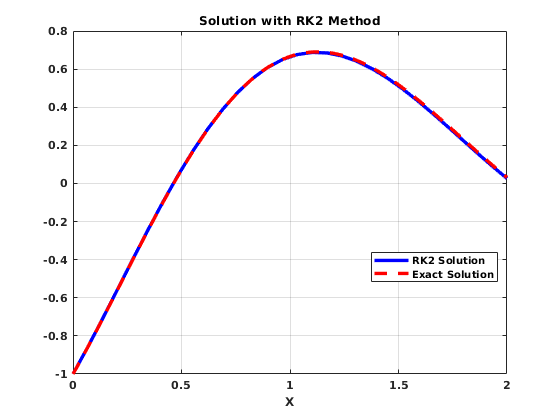
\includegraphics{lec25n-ex2.png}
\caption{Solution of Example \#2.}
\label{fig:lec25n-ex2}
\end{marginfigure}
\begin{marginfigure}
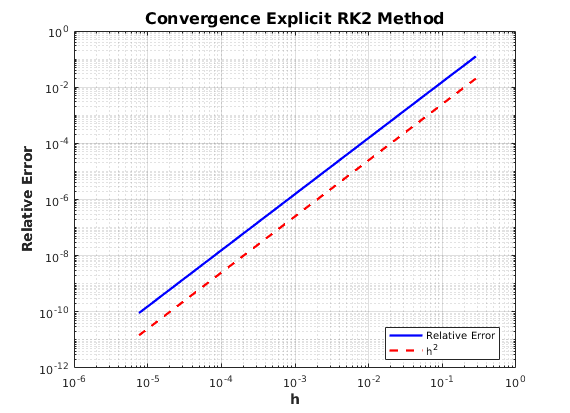
\includegraphics{lec25n-ex2-conv.png}
\caption{Convergence behavior of 2\textsuperscript{nd}-order RK solver for systems of equations.}
\label{fig:lec25n-ex2-conv}
\end{marginfigure}
The solution of Example \#2 is shown in Figure \ref{fig:lec25n-ex2} and the convergence behavior of the 2\textsuperscript{nd}-order RK solver for systems of equations is shown in Figure \ref{fig:lec25n-ex2-conv}.




